\documentclass{article}
\usepackage[margin=2.5cm]{geometry}
\usepackage{amsmath, amssymb, stmaryrd, latexsym, amsthm, mathtools}
\usepackage{mathpazo, times}
\usepackage{float}
\usepackage{listings}
\usepackage{url}
\usepackage{natbib}
% \usepackage{parskip} % very ugly with lemmas, invariants, etc without intervening text
\usepackage[disable]{todonotes}
\usepackage{slashed}
\usepackage{tikz}
\usepackage{forest}
\usepackage{IEEEtrantools}
\usepackage{microtype}
\usepackage{graphicx,color}

\usepackage{hyperref}
\hypersetup{
  colorlinks=false,
  linkcolor={blue},
  citecolor={blue},
  urlcolor={blue},
  linkbordercolor={white},
  citebordercolor={white},
  urlbordercolor={white}
}
\usepackage[capitalise,noabbrev,nameinlink]{cleveref}

% https://tex.stackexchange.com/questions/132823/ieeetrantools-clash-with-cleveref
\makeatletter
\let\if@IEEEissubequation\iffalse
\makeatother

\usetikzlibrary{arrows}

\newcommand{\njd}[1]{\textcolor{purple}{\emph{#1}}}
\newcommand{\avieth}[1]{\textcolor{blue}{\emph{#1}}}
\addtolength{\marginparwidth}{-0.1\marginparwidth}

\newcommand{\powerset}[1]{\mathbb{P}(#1)}
\newcommand{\order}[1]{\mathcal{O}\left(#1\right)}
\newcommand{\restrictdom}{\lhd}
\newcommand{\subtractdom}{\mathbin{\slashed{\restrictdom}}}
\newcommand{\restrictrange}{\rhd}

\DeclareMathOperator{\dom}{dom}
\DeclareMathOperator{\range}{range}
\DeclareMathOperator*{\argmin}{arg\,min} % thin space, limits underneath in displays
\DeclareMathOperator*{\minimum}{min}
\DeclareMathOperator*{\maximum}{max}

% Number within sections, and don't have separate counters for separate environments
\theoremstyle{definition}{
  \newtheorem{lemma}{Lemma}[section] % Number within sections
  \newtheorem{definition}[lemma]{Definition}
}
\theoremstyle{theorem}{
  \newtheorem{invariant}[lemma]{Invariant}
  \newtheorem{proofobligation}[lemma]{Proof Obligation}
}

\Crefname{invariant}{Invariant}{Invariants}

\numberwithin{equation}{lemma}

\floatstyle{boxed}
\restylefloat{figure}

\lstset{basicstyle=\ttfamily\small}

\raggedbottom

\begin{document}

\title{Design of IPC protocols for Cardano Shelly \\
       {\small (Version 0.2)} \\
       {\large \sc An IOHK technical report}}
\author{Duncan Coutts \\ {\small \texttt{duncan@well-typed.com}} \\
                         {\small \texttt{duncan.coutts@iohk.io}}
   \and Alex Vieth \\ {\small \texttt{alex@well-typed.com}}
   \and Neil Davies \\ {\small \texttt{neil.davies@pnsol.com}} \\
                       {\small \texttt{neil.davies@iohk.io}}
   }
\date{June 22, 2018}

\maketitle

\begin{abstract}
This document is intended as a discussion, leading to a design, of IPC
protocols for Cardano's Shelly release. The structure of the discussion is to
look at the requirements and ideas for application-level protocols, before
looking at how those can map onto lower level IPC protocols.
\end{abstract}

\tableofcontents

\section*{Version history}

\begin{description}
\item[Version 0.1, June 18, 2018] First draft based on previous notes and
                                  discussions with Alex.
\item[Version 0.2, June 22, 2018] Sketch of protocol proposal and goals for
                                  how to elaborate, based on further review
                                  and discussion with Alex and Neil.
\end{description}

\section{Introduction}

\subsection{Scope}

In scope for this discussion is IPC that Cardano nodes engage in. We do want
to consider IPC between Cardano nodes and components such as wallets and
explorers, but not between wallets/explorers and other components.

Part of the discussion will be motivated by algorithms, data structures and
resource constraints within nodes, such has how nodes can represent their
blockchains, but this document is not primarily an analysis of those issues.

There are two relatively clearly distinct use cases for IPC for Cardano nodes:
\begin{itemize}
\item IPC between Cardano nodes that are engaged in the high level Ouroboros
      blockchain consensus protocol.
\item IPC between a Cardano node and a `chain consumer' component such as a
      wallet, explorer or other custom application.
\end{itemize}

It is plausible that both use cases could be served by the same protocol, but
this is not a given a priori.

\subsection{Goals}

First and foremost the protocols need to achieve their information exchange
requirements.

For the node-to-node protocol this is driven by the functional and performance
needs of Ouroboros. The node-to-node protocol is conducted in a P2P environment
with very limited trust between peers. The node-to-node protocol utilises
store-and-forward over selected \emph{bearers} which form the underlying
connectivity graph. A concern in this setting is asymmetric resource consumption
attacks. Ease of implementation is a nice to have, but is subordinate to the
other hard constraints.

A node-to-consumer protocol is intended to support blockchain applications
like wallets and explorers, or Cardano-specific caches or proxies. The setting
here is that a consumer trusts a node (a `chain producer') and just wants to
catch up and keep up with the blockchain of that producer. It is assumed that
a consumer only consumes from one producer (or one of a related set of
producers), so unlike in the node-to-node protocol there is no need to choose
between different available chains. The producer may still not fully trust the
consumer and does not want to be subject to highly asymmetric resource
consumption attacks. In this use case, because of the wider range of
applications that wish to consume the blockchain, having some options that are
easy to implement is more important, even if this involves a trade-off with
performance. That said, there are also use cases where tight integration is
possible and making the most efficient use of resources is more desirable.

\subsection{Why distinguish node-to-consumer}

It is worth discussing briefly why it makes sense to consider a node-to-consumer
protocol distinct from a node-to-node protocol.

There are a number of applications that simply want to consume the blockchain,
but are able to rely on an upstream trusted or semi-trusted Cardano consensus
node. These applications do not need to engage in the full consensus protocol,
and may be happy to delegate the necessary chain validation.

Examples include 3rd party applications that want to observe the blockchain,
examples being business processes triggered by transactions or analytics.  It
may also include certain kinds of light client that wish to follow the
blockchain but not do full validation.

Once one considers a node-to-consumer protocol as a first class citizen then it
opens up opportunities for different system architecture choices. The
architecture of the original Cardano Mainnet release was entirely homogeneous:
every node behaved the same, each trusted nothing but itself and paid the full
networking and processing cost of engaging in the consensus protocol.  In
particular everything was integrated into a single process: the consensus
algorithm itself, serving data to other peers and components such as the wallet
or explorer. If we were to have a robust and efficient node-to-consumer protocol
then we can make many other choices. \marginpar{\njd{Process memory space as
    the basis of trust}}.

With an efficient \emph{local} IPC protocol we can have applications like
wallets and explorers as separate processes. Even for tightly integrated
components it can make sense to run them in separate OS processes. Not only is
the timing constraints for a consensus node are much easier to manage when it
does not have to share CPU resources with chain consumers, but it enables the
use of operating system features to give finer control over resource consumption
for sophisticated end-users.
There have been cases in production where a highly
loaded wallet component takes more than its allowed allocation of CPU resources
and causes the local node to miss its deadlines.  By giving a consensus node a
dedicated CPU core it becomes more plausible to provide the necessary hard real
time guarantees. In addition, scaling on multi-core machines is significantly
easier with multiple OS processes than with a multi-threaded OS process with a
shared-heap. This could allow for larger capacity Cardano relay deployments
where there are multiple network facing proxy processes that all get their chain
from a single local consensus node.

With an efficient \emph{network} IPC protocol we can do similar things but
extend it across multiple machines. For example, clusters of relays operated
by a single organisation may be also to operate more efficiently using a
node-to-consumer protocol than a node-to-node protocol. Similarly it allows for
wallet or explorer-like applications that need to scale out, and are able to
make use of a trusted node.

\njd{In someways what is being proposed here is that by creating the notion of
  a `chain-observer' we can gain flexibility, reduce both computational and
  space complexity and enable a range of `lighter-weight' products and derived
  services.
  }

\section{Node-to-consumer protocols}

TODO: cover notes on:
\begin{itemize}
\item chain producer representations and in-memory storage with high degrees of forking
  \begin{itemize}
  \item bounds on likely forking numbers, thus bounding the attack surface,
    likely to susceptible to analysis via some (pretty simple - i.e have
    analytical solutions) Markov Chain models.
    \item use-cases
  \end{itemize}
\item chain producer keeping state about consumers
\item immutable vs volatile distinction in representation and protocols
\item stateful protocol
\item stateless protocol
\item recursion as an indicator of completeness \marginpar{\njd{what does this mean Duncan?}}
\item family of protocol variations for different environments: STM, IO, local
  IPC, remote IPC
  \njd{\\noting different levels of implict trust here - we need
    to think whether the STM enviroment is one we treat differently (e.g. trust
    forwarding only correctly signed blocks reducing the checks in the consumer
    end) or do we assume even shared process nodes are potentially missbehaving
    and play up the way in which that helps defend against other forms of attack? }
\item optimised case for immutable chain, e.g. shared files
\item STM interface
\item coping with talking to a load-balanced cluster of imperfectly synced producers
\end{itemize}

\section{Node-to-node protocol}

The Ouroboros consensus protocol \citep{ouroboros-classic} describes what it
needs from its network layer. That is:
\begin{itemize}
\item nodes that create a new block in a time slot need to be able to broadcast
      their \emph{entire blockchain} to all other nodes, and;
\item within each time slot, all nodes to collect \emph{all the blockchains}
      they have received via broadcast and then to pick among them.
\end{itemize}

The challenge is to simulate this specification in bounded resources and to do
so without opening up opportunities for new attacks at the network level. Such
attacks might include preventing broadcast or local denial of service by making
them consume excess resources (time, memory, network, CPU).

Obviously na\"ively broadcasting entire chains is not something that can be
done with bounded resources since there is no bound to the chain length.
Obviously the intention is to communicate new blocks and to share and reuse the
parts of the chain that have not changed, though this is easier said than done.

There is however another dimension to the resource bounding problem. In a
proof-of-work blockchain protocol it is expensive for adversarial parties to
create lots of `fake' blocks, so there is in practice a limit on the number of
such blocks that honest parties need to consider. In proof-of-stake blockchain
protocols there is no such constraint: adversarial parties can create many
signed blocks.

\subsection{Drawbacks in the current Ouroboros network protocol implementation}

In the current architectural deployment there is an assumption that certain
nodes are being run by trusted parties and, as such, non-adversarial. There is
no current formal argument as to how, in the presence of nodes acting
adversarially with respect to data diffusion, at what level of adversarial
action performance is compromised.

\subsection{Broadcasting versus subscribing}

It is tempting to consider pursuing an approach where each node subscribes to
and follows the chains of a number of its peers and continuously selects
between those chains following the Ouroboros chain validity and longest chain
rules. This would allow us to impose constraints such as that each node only
announces a single new block to its peers in each slot, since it would only be
announcing the head of its own adopted chain. That obviously makes it easier
for a node to bound its resource use since it only need consider N potential
chains from the N peers it is subscribed to.

It is not clear however that this is equivalent to what Ouroboros specifies:
that chains be broadcast to everyone, and that each node looks at all chains
that it receives within each time slot. By contrast the equivalence argument is
much clearer if we broadcast the block header of each chain's head (via
multicast or flooding over point-to-point links), and then chase down the rest
of the chain back to an intersection point.

We will restrict ourselves to algorithms that can plausibly be argued are
equivalent to broadcasting chains.

\subsection{Trying to bound Ouroboros bearer, compute and storage resource use}

There are a few aspects to bounding resource use in this distributed setting.
\begin{enumerate}
\item We can try to establish some absolute bound on the required resources.
\item With or without an absolute bound we can try to arrange things so that it
      is difficult for an adversarial party to create a lot of work for honest
      parties.
\item If we cannot establish absolute resource bounds for a perfect simulation,
      or the bounds might be too large for some instances, we can consider what
      choices an instance with limited resources should make to achieve a good
      enough simulation.
\end{enumerate}

Let us review ideas on each point in turn.

\subsubsection{Trying to establish absolute bounds}

There are a number of standard tricks here. For starters we can break up the
blockchain into individual blocks, and blocks themselves into a small fixed
size header and a larger variable sized body. The basic idea is then that we
initiate a chain broadcast by broadcasting the block header for the head block
in the chain.

In PoW blockchain algorithms the header can contain the representation of a
proof of work, while in PoS the header contains representation of the proof of
stake: a signature showing that it was created by the appropriate party. In
Ouroboros the PoS signature means that nodes that are up to date (at least
within the same epoch) can verify that the header itself is plausible, and
exclude incorrectly signed or inplausible headers.

A small fixed size header means that we can bound the network resource use
to send or receive a single header, and can also bound the CPU resources needed
to verify the header.

Additionally the Ouroboros algorithm imposes a number of useful constraints:
\begin{itemize}
\item Ouroboros specifies that chains with blocks from slots in the future are
      invalid. The signed block header contains the slot number so we can
      exclude such chains just by looking at the block header of the head block
      in the chain (which is the one we broadcast).
      \avieth{If a slot leader can mint a new block and deliver the header to
      a peer within the clock skew of that peer then it may be incorrectly
      rejected. We may want to set some tolerance threshold.}
\item Ouroboros specifies that when a node adopts a new chain it only ever
      picks one strictly longer than its current one. The signed block header
      contains the block number so by comparing the block number of the
      broadcast header against the current length of the node's chain, we can
      exclude chains that are shorter and so could never be picked.
      \avieth{Further, it is never necessary for a node to relay a chain when it
      knows of a better one. This may be very useful in practice: at most one
      chain must be tracked per peer. An adversary cannot make an honest node
      retain multiple chains of its own broadcast.}
\item Ouroboros classic (but not BG\marginpar{\njd{first use - expand}}) specifies that a node will only ever pick
      a chain that diverges from its current chain within the last K blocks,
      implying that forks can be at most K long. This places a bound (of K) on
      the range in which a node needs to look for an intersection between the
      new purported chain (represented by the header of its head block) and its
      own current chain. This bounds the number of block headers that a node
      would ever need to download to obtain all headers for the candidate chain.
\item Each block must be signed by the appropriate slot leader. This signature
      -- which is the proof of stake -- can be checked by any node that has
      the chain up to the current epoch.
\item In Ouroboros classic, there is only ever one legitimate leader for each
      time slot, and non-adversarial players never sign more than one block
      for the slots in which they are the leader.
\item In Ouroboros BG, the situation is similar: there can be more than one
      legitimate leader for a time slot but the number of leaders in a slot
      follows a distribution that makes a large number highly unlikely (and
      this is not controlled by adversarial players).
\item In both Ouroboros classic and BG it is possible for adversarial players
      to sign multiple blocks for the same slot, but this is visible (so-called
      `open adversarial behaviour').
\item \avieth{Theorem 4.13 from the original Ouroboros paper describes the
      probability of the existence of a flat fork of length $n$: 2 tines of
      equal block count intersecting $n$ slots prior. This is applicable to
      what we're doing here, both for resource bounds and for correctness.}
\end{itemize}

The combination of these constraints does place a limit on the number and
length of plausibly valid chains that an adversary can create and try to get
honest parties to chase. Given that some honest parties may have gone offline
and be a long way behind the chain, and in particular will not be able to
validate signatures in block headers. So it is worth splitting the analysis
into the case of nodes that are within the current epoch, and a case for nodes
that are further behind. We start with the first case.

In particular, plausibly valid chains would have to start with a valid header
that falls into a slot after the last block of the target victim's chain
but only up to the current time slot. Plausibly valid chains can only extend
back up to K blocks (max 2K slots). The victim is able to assume that other
honest nodes do not sign more than one block per slot, this imposes the
constraint that the adversary can only send one header per slot within the
range just described.
\avieth{Why? I don't see it. Plausibly valid chains can extend more than
  K blocks, no? Maybe the language is unclear.}

It is worth noting that just because honest nodes do not sign more than one
block per slot, it does not mean that different honest nodes will not have
different blocks in the same slot, since an adversary can in previous slots
have sent different headers to different nodes.

\njd{\centering I'm not certain I agree with this, or perhaps I don't agree
  with the implied generality. Honest generator nodes will only generate one
  block per slot - so only one of those can exist per slot. Dishonest nodes can
  generate many such blocks, agreed - maybe that needs to be brought out.}

\avieth{What's the disagreement here?}

\paragraph{An overall bound} Suppose the victim node has a chain with
at least $K$ blocks covering the last $K \leq s \leq 2K$ slots, and $n$ slots
between the slot of the head block of chain on the victim node's and the
current time slot. Suppose also that the adversary controls a fraction
$0 \leq \rho < 1/2$ of the stake in the current epoch.

In that case the adversary can create approximately $n * \rho$ chains (the
specific slots in which the adversary is leader is drawn from a probability
distribution). In the worst case this approaches $n / 2$, but of course the
adversary is allowed to wait until it gets lucky in the probability
distribution. Each of these chains can be up to approximately $(n+K) * \rho$
long. Of course only the chains that are actually longer than the victim node's
current chain are valid.

\njd{This would seem to be the right spot for the simple MC analysis on
  distribution of burst lengths\\
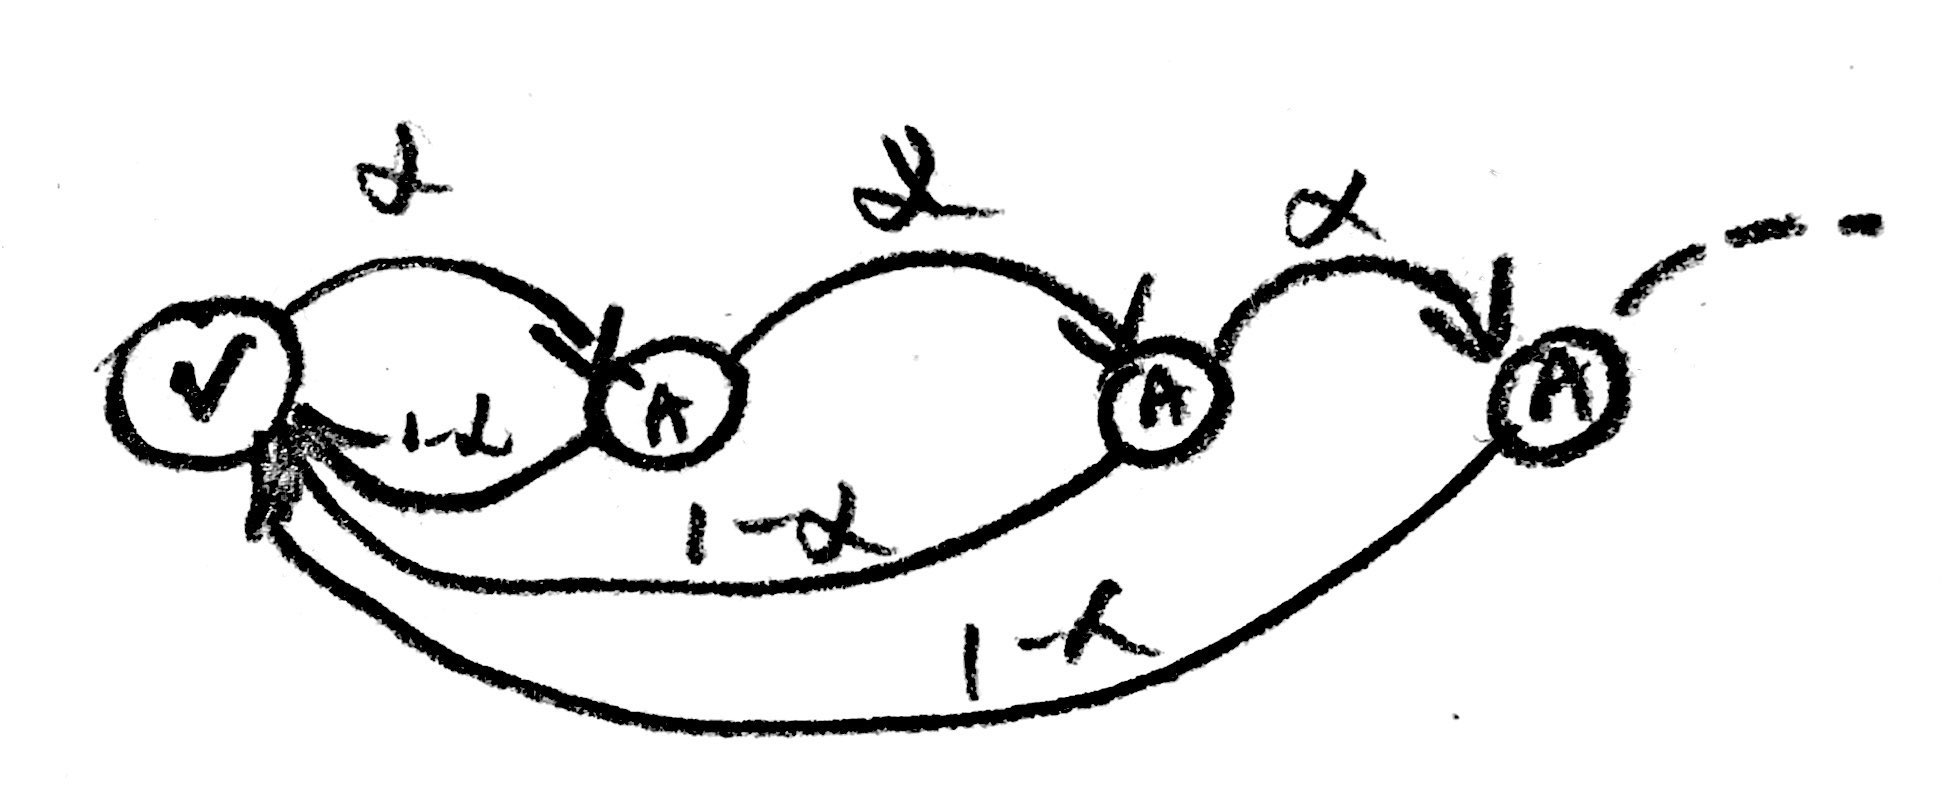
\includegraphics[totalheight=2cm]{burst-length-mc.png}}

\avieth{Proposal for a data structure for forks over $k$ slots.}

\avieth{For each peer to which the node is connected, at most one chain (their
  claimed best chain) is retained. An honest node only broadcasts or relays
  a tip-of-chain if it has judged it to be the best chain it knows. There is
  no reason to broadcast or relay any other chain: by broadcasting or relaying
  the better chain, the honest receiving party will always prefer it to the
  weaker one, so broadcasting or relaying the weaker one would be wasteful.}

\avieth{When a tip-of-chain announcment is received from a peer, and it's valid
  (signed by the appropriate slot leader) and better (higher block count) than
  the peer's previously announced best tip-of-chain (if any), the receiver
  either:}

  \begin{itemize}
    \item \avieth{If the parent of the header is known, and it is also the tip of the
          local node's best chain, then the new header can be relayed
          immediately. The peer will send the body as well which can also be
          relayed immediately upon reception.}
    \item \avieth{If the parent of the header is not known, some protocol to find
          the intersection is engaged. It could be a naive request for headers
          of ancestors, or something more complicated such as the one described
          in the ``A protocol proposal" section of this document. In any case,
          eventually either the intersection is found and the complete peer's
          chain downloaded (up to at most $k$ blocks), or the peer fails to
          provide enough information and the chain is eventually discarded.}
  \end{itemize}

  \avieth{A loose upper bound on space use is the number of peers multiplied by $k$.
  As for network I/O and CPU resource use: an adversary can only induce an
  honest node to work on one chain, namely the adversary's claimed best chain.
  By judiciously queueing network input we can ensure that adversaries cannot
  cut out honests.}

  \avieth{The probabilty that a node has multiple chains which disagree on the
  slot $n$ behind the current slot is marginal for sufficiently large $n$
  (theorem 4.13). This gives a local correctness property: by increasing the
  number of slots retained by this forking data struture ($k$) we can
  decrease the probability that the oldest slot will include more than one
  candidate (mutiple blocks, or no block, because some maximal chain is known
  with no block at this slot). Multiple candidates for the oldest slot means
  there is a flat fork of size $k$: 2 tines of equal block count intersecting
  at the slot $k$ behind the current slot. This is highly unlikely for high
  $k$ (negative exponential in $k$).}

  \avieth{As for consistency between peers: if 2 nodes disagree on the slot $k$ behind
  the current slot, it's not necessarily a flat fork: one of the chains could
  have a lower block count than the other, which means the disagreement is due
  to communication failure. In particular, the peer with the better chain
  failed to broadcast its chain to the peer with the weaker chain. In order to
  get some guarantee on inter-node consistency, we might use properties of
  the network, perhaps some $\Delta Q$ analysis.}

  \avieth{Call the better tine $T_b$ and the worse $T_w$. $T_b$ has a higher
  block count $bc(T_b)$ than $T_w$, so there is some subchain of $T_b$ which is
  a flat fork of $T_w$, obtained by removing the $bc(T_b) - bc(T_w)$ newest
  blocks from $T_b$. The size of this flat fork is probably very small
  (theorem 4.13). If the disagreement is for a block $k$ behind the current
  slot then, since this flat fork is probably small, the difference
  $bc(T_b) - bc(T_w)$ must be comparatively large, and so the node with the
  better chain must have had a comparatively high number of slots in which
  it could have informed the node with the weaker chain of its better chain.
  This is informal but I think it captures the idea and we may be able to
  work it into some explict probabilistic guarantee.}

\subsubsection{Raising the difficulty for attackers}

As designers of the protocol game we want to structure it such that the
defending party can make best use of the available bounds so that the attacking
party cannot do much better than those bounds. In this case that means trying
to avoid consuming too much network or other resources downloading chains that
we will later discover are invalid. Attacking nodes can lie, and we must
structure the game so that we can catch them out on the lie within bounded and
reasonable resources.

There are a few observations we can make from the above bounds. Firstly,
nodes that are further behind are much more vulnerable since there are many
more starting points for potential chains that an attacker can use.

An important observation is that attackers with a lower stake proportion $\rho$
can initially claim that they have a candidate chain that is longer than the
victim's chain and that intersects with it many blocks back, but they will not
be able to substantiate that claim. That is because the attacker can only make
signed block headers for the slots it controls. They can use slots they control
within the $n$ slots between the victim's chain head and the current time slot,
but the further back the attacker tries to make the intersection, they soon
run into the problem that the density of chain they can create is much lower
than the density of the victim's chain. So while the attacker has an $n * \rho$
head start, they soon loose out in trying to construct a valid chain.

Given that the attacker can lie, we wish to structure the game so that we can
catch them out on the lie with a minimum use of resources by the victim. We can
use techniques such as requiring the attacker to reveal more information up
front making it easier for the victim to detect the lie later, and we can use
tricks like making certain challenges randomly so that the attacker cannot pick
a perfect strategy up front.

\subsubsection{Judicious choices on resource use}

If the resource bounds are in the worst case still more than the available
resources of the instance of the implementation, we may still be able to
make adequate progress. If so, it involves deciding carefully which options
to pursue and which to pass up. This requires careful analysis 

\subsection{A protocol proposal}

In this section we will propose a protocol at a high level with a general
description of the algorithm that the defending party can follow.

We need to analyse this protocol in at least the following cases
\begin{itemize}
\item A high stake adversary: one that can construct multiple long enough valid
chains according to the bounds, and many other plausible long but ultimately
invalid chains.
\item A low stake adversary: there are many more low stake adversaries than
high stake ones, so this is an important case. We need to be sure we can deal
with multiple low stake adversaries quickly.
\item A low or zero stake adversaries that rely not on signing their own blocks
but on grabbing real valid signed blocks and trying to cause mischief with
them. For example, the algorithm should deal efficiently with an attacker that
simply re-broadcasts many valid headers from the current chain.
\item The protocol game we create is reversible: whatever protocol we define
we must consider in both directions, either side can be the honest node with
the other the adversary. We must analyse the resource use from the broadcast
side as well as the receiving side.
\end{itemize}

The sketch of the protocol is as follows:
\begin{enumerate}
\item The (potential) adversary sends a new block header messages.
      The block header message contains a signed block header (roughly ~600
      bytes) and a list of pairs of slot number and hash of a predefined
      set of preceding blocks on their chain. We could use e.g. 16 immediately
      preceding and then ${2^n | n \in {5..15}}$ blocks earlier. This is an
      initial declaration by the attacker and can be used to find the lower
      bound on the purported chain intersection point. The purpose of providing
      the first few densely is to deal efficiently with the common and
      non-adversarial cases of follow-on blocks or short forks.
\item The defender must check the block signature and discard it if it is
      invalid. Honest nodes should never forward invalid signed blocks so this
      indicates the immediate peer\marginpar{\njd{the direct bearer peer}} is dishonest and should be dropped.
\item Assuming the block signature is valid, and it's slot number and block
      number indicate it is of interest, the node must now remember the slot
      and hash of this block header since any other validly signed block header
      in this slot indicates both broadcasts were adversarial and can be
      ignored. The node can also now re-broadcast this header to its other
      peers that are subscribed.
\item The defender, by looking at the purported points on the new chain can now
      determine a lower bound on where the chain intersection would be (or that
      there is none and it can be discarded). This is true because the points
      on the chain cover up to one epoch back.
\item The defender now issues a request containing a set of block numbers (or
      offsets backwards from the chain head) on the attackers chain. The
      request is for the corresponding slot numbers and block header hashes.
      These can be made quite small, e.g. the first 64bits of the block hashes\marginpar{\njd{they could be even smaller? what risk in 8, 16 or 32 bits?}}.
      The purpose of this request is to force the attacker to reveal
      information up front so that it cannot take an adaptive approach to our
      later requests. If the range that the defender is interested in is too
      big for a single request, it should pick points (or ranges of points?)
      randomly. \\ \njd{If smaller hashes are not that much weaker this might help with message sizes at this point}
\item The attacker now sends the slot numbers and block header hashes, or the
      request times out, and the defender can stop chasing this chain. Note
      that this does not indicate the immediate peer is an adversary since we
      re-broadcast headers prior to validating the whole chain of headers.
\item The defender can now ask for a selection of block headers, based on the
      block numbers they asked for previously. Block headers are a bit larger
      so we can only ask for fewer than in the previous request. The defender
      should ask for points on the chain randomly. This is to prevent the
      attacker from using the slots they do control in a strategic way.
\item The attacker must supply the headers requested (or abandon).
\item The defender can now validate these headers and check them against the
      slot numbers and hash prefixes previously declared by the attacker. The
      argument is that if the attacker in fact can only sign a proportion of
      the slots they are claiming (or cannot make the links or block numbers
      match up), then by repeatedly sampling them randomly the defender has
      a very high chance of catching them out in the lie, without having to
      download the whole purported chain. The smaller the adversarial stake
      $\rho$ and the longer the claimed fork the greater the chance of catching
      the lie quickly.
\item The defender can iterate asking for more block headers (and if it was
      necessary more slot numbers and block header hashes) until either an
      invalid header chain is discovered or all the headers from the
      intersection point to the chain head are found. It may be appropriate
      (if the analysis allows) to use larger batches for subsequent requests
      as the probability of a lie dwindles.
\item Once the defender has established a full chain of headers, it can request
      the block bodies, either from the same node or from any other peer.
\item Finally it can apply the new chain to its chain state if it is still
      longer than its current chain.
\item It is important to abandon this protocol if it takes too long overall.
      A single slot-worth of time may be appropriate. \\ \njd{maybe this should be a progress condition not an abandonment. What would the mitigation action be if abandoned? - restarting could bery well be exactly the wrong thing to do - i.e can we structure the protocol interactions so assure monotonic progress}
\item It is important to retain valid signed headers in a cache, even if the
      chain chasing was abandoned due to a timeout. This is because while an
      attacker can make lots of different invalid chains that are all wildly
      divergent, the honest chain gets built upon, so if we are in a situation
      where we are trying to chase many possible chains, while we may not be
      able to complete the chasing of the honest chain within the timeout we
      can hopefully make progress on it at better than real time, and so b
      remembering it from slot to slot we can build on it and eventually chase
      down the whole chain of headers. It is not necessary to retain headers
      when the chain was discovered to be invalid.
\end{enumerate}

TODO: need better name than attacker here, since the immediate peer may be
honest and just be proxying for the real attacker. This is due to us wanting
to broadcast headers before waiting for the full chain to be validated.\\
\njd{fuzzy logic here we come? or some Bayesian reasoning approach?}
\avieth{How's this: only relay the header immediately if its parent chain is
  already known and valid? Then we get a speedup for the typical case: relaying
  a block freshly minted by an honest slot leader. In other cases, it won't be
  relayed until it has been downloaded and verified.}

TODO: during this whole process, the chain state may have updated already and
the chain we're chasing may be redundant.

TODO: consider priority between the chains we're chasing, e.g. when we get a
full chain of headers, dedicate the bandwidth to fetching the blocks rather
than chasing more? Do it adaptively as the lie probability dwindles? Or does
that dangerously favour short adversary chains over genuine longer ones? \\

\njd{If we tie key resource consumption ratio - thinking mainly
  network resource here - to fractional belief and we only manipulate
  ratios not preemption (i.e weight not pitch) then a short-chain
  attacker who dawdled would free up resources for a longer one to
  overtake it. We may be able to make this a non-problem.}

\bibliographystyle{apalike}
\bibliography{references}

\appendix
\section{Credible worst case scenario(s)}
\subsection{Bounding case}
\begin{itemize}
\item attacker can totally eclipse node
\item attacker has  $\rho = \frac{1}{2} - \epsilon, \epsilon > 0$ stake
\end{itemize}
\subsection{Duration of miss-information}
\begin{itemize}
\item how many slots could an attacker maintain a fiction with a)
  unfettered power of eclipse; b) $\rho$ adverserial stake at its disposal.
\item what indicators of certainty are available to inform end user?
\end{itemize}
\subsection{Inherent Assymetry}
\begin{itemize}
\item How much un-eclipsed information is needed to detect eclipse? Is
  a unicast channel enough? (this would permit other technological
  approaches in the longer run)
\item Given that a node is not totally eclipsed (i.e $\exists$
  potentially reachable non-adversrial bearer node) how does this help?
\end{itemize}  


\end{document}
